\chapter{Problém množinového pokrytia a výber génov}
\label{chap:setcover}
V predchádzajúcej kapitole sme si predstavili základné prvky nášho programu ktorý dostane na vstupe súbor, 
popisujúci evolučnú históriu a na výstupe nám vykreslí fylogenetický strom reprezentujúci danú históriu.
Problém nastane, pokiaľ v histórii nachádza príliš veľa génov. Výsledný vygenerovaný obrázok sa stáva neprehľadným, 
a získanie informácie z neho obtiažne. 
Potrebujeme teda vybrať iba niektoré gény na zobrazenie tak, aby na obrázku zostali zachované podstatné informácie.
V tejto kapitole si predstavíme spôsob, akým budeme vyberať ktoré gény zobrazíme,
využitie \emph{Problému množinového pokrytia} pri hľadaní daných génov a dva algoritmy ktoré riešia daný problém.
\section{Výber génov}
Najpodstatnejšou informáciou pri analýze fylogenetického stromu je pre nás to, aké udalosti sa v ňom odohrali. 
Budeme sa teda snažiť nájsť podmnožinu všetkých génov tak, aby všetky udalosti ostali na obrázku zachované.
Zvyšné gény následne z obrázku odstránime, čo môže viesť k strate informácií ktoré považujeme za menej podstatné, 
ako napríklad to, koľko a ktoré geńy sa nachádzajú v danej histórii, ako aj koľko a ktoré gény sú ovplyvné danou udalosťou.
\subsection{Blok}\label{blok}
\emph{Blok} predstavuje postupnosť génov ktoré sa pred aj po kroku e.h. nachádzali vedľa seba v rovnakom poradí a jednotlivé gény nemenili svoju orientáciu. Jedná sa teda o súvislý
úsek DNA ktorý počas kroku e.h. nebol prerušený.
Ak sa pri delécii alebo inzercii odobralo alebo pridalo viacero génov, a nenachádza sa medzi nimi žiaden iný gén, tvoria jeden blok.
Pri duplikácii gény tvoria blok ak sa nachádzali pri sebe pred duplikáciou a rovnako aj po nej vo všetkých zduplikovaných inštanciách.
Pri Inverzii sa gény nachádzajú v bloku pokiaľ sa všetkým zmení orientácia, t.j. zrotuje celý blok.
Napr blok génov (4,5,-6) bude po inverzii vyzerať ako (6,-5,-4).
\begin{figure}[t]
 \centering
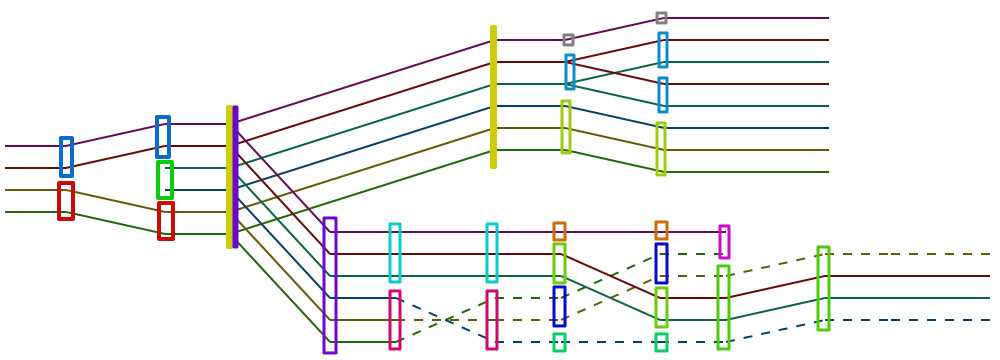
\includegraphics[width=1\textwidth]{images/bloky}
\caption{Ukážka blokov.}\label{obr:bloky}
\end{figure}
\subsubsection{Pokrytie blokov}
Blok považujeme za pokrytý pokiaľ sa na obrázku vyskytuje aspoň jeden gén patriaci do daného bloku.
Pokrytie všetkých blokov jedného kroku e.h nám zaručí zobrazenie všetkých udalostí, aj keď nie v úplnom rozsahu,
ktoré sa v danom kroku vyskytli.
Musíme preto nájsť také gény, ktoré pokryjú všetky bloky v kompletnej evolučnej histórii,
a tým si zaistiť zobrazenie všetkých udalostí vo výslednom fylogenetickom strome. 
Ako cieľ si zvolíme aby bola daná množina génov čo najmenšia.
\section{Problém Množinového Pokrytia}
\paragraph{Definícia}
Máme dané univerzum$U$, ktoré obsahuje $n$ prvkov, a systém jeho podmnožín \(S=\{ P_i : P_i \subseteq U \}\), 
ktorý pokrýva celé univerzum \(\cup_{Pi \epsilon S} Pi = U\),
vybrať čo najmenšiu množinu podmnožín \(C \subseteq S\)
takú ktorá tiež pokryje celé Univerzum \(\cup_{Pi \epsilon C} Pi = U \) .\\
Problém Množinového Pokrytia (anglicky Set Cover Problem), ďalej len \emph{PMP}. patrí medzi NP-úplne problémy.\cite{Karp}
\paragraph{Príklad}
Pre Univerzum$U=\{1,2,3,4,5,6\}$ \\a systém jeho podmnožín
$S=\{\{1,2,3\},\{2,3\},\{3,4\},\{3,4,6\},\{5\}\}$ \\
je riešením množina podmnožín $C=\{\{1,2,3\},\{3,4,6\},\{5\}\}$ 
\subsection{Výber génov pomocou Problému Množinového Pokrytia}
Výber takých génov ktoré pokryjú všetky bloky v celej evolučnej histórii vieme formulovať
ako Problém Množinového Pokrytia 
Univerzum predstavuje všetky bloky ktoré sa nachádzajú v našom fylogenetickom strome.
Každý gén predstavuje jednu podmnožinu, v ktorej sa nachádzajú tie bloky, cez ktoré gén prechádza.
Riešením je taká množina génov, ktorých zjednotenie pokrýva všetky prvky Univerza, v našom prípade všetky bloky nachádzajúce sa v evolučnej histórii.
\section{Riešenie Problému Množinového Pokrytia}
Keďže \emph{PMP} patrí medzi NP-ťažké problémy, znamená to že zatiaľ neexistuje,
a možno nikdy ani nebude existovať algoritmus ktorý by dokázal nájsť riešenie v polynomiálnom čase.
Potrebujeme sa teda rozhodnúť, či je pre nás výhodnejšie hľadať najlepšie riešenie \emph{PMP} 
čo môže byť časovo náročné,
alebo sa uspokojíme s približním riešením, ktoré sme schopný nájsť aproximačným algorimtom v polynomiálnom čase,
a ktoré môže taktiež predstavovať dostatočné odstránenie prebytočných génov z obrázku.
Predstavíme si jeden spôsob ktorým budeme hladať úplné riešenie, jeden spôsob na nájdenie približného riešenia a v
nasledujúcej kapitole porovnáme výsledky ktoré produkujú. 
\subsection{Greedy algoritmus}
Greedy algoritmus patrí medzi najlepšie polynomiálne aproximačné algoritmy pre riešenie \emph{PMP}.\cite{Slavik}
Greedy algoritmus v každom kroku pridá do riešenia takú podmnožinu,
ktorá obsahuje najviac zatiaľ nepokrytých prvkov univerza. Riešenie teda hľadáme nasledovným spôsobom:\\
% Peter Slavik A tight analysis of the greedy algorithm for set cover %citation
Všetky podmnožiny zoradíme na základe toho, koľko prvkov obsahujú.
Do riešenia vyberieme najvačšiu podmnožinu a prvky, ktoré sa v nej nachádzajú odstránime z
univerza aj zo zvyšných podmnožín. Zvyšné podmnožiny opäť zoradíme podľa veľkosti,
a postup opakujeme až pokým nie je Univerzum prázdne.\\
Tesná analýza podľa Slavíka ukazuje, že aproximačný koeficient takéhoto riešenia je \(\ln m - \ln \ln m\ +\Theta(1) \) \cite{Slavik} 
kde \(m = |U|\).
\subsection{Binárne-Celočíselné Lineárne Programovanie}
\label{sub:bclp}
Lineárne programovanie je optimalizačná úloha, pri ktorej je cieľom nájsť minimum alebo
maximum lineárnej funkcie $f$ s $n$-premennými, zatiaľ čo máme dané lineárne obmedzenia vo forme rovníc a nerovníc.
V prípade binárneho-celočíselného lineárneho programovania nadobúdajú premenné hodnotu 0 alebo 1,
a všetky atribúty obmedzujúcich rovníc a nerovníc sú celočíselné.
Binárne-Celočíselné lineárne programovanie (angl: 0-1/binary integer linear programming),ďalej BILP patrí medzi NP-úplné problémy.\cite{Karp}
Množstvo iných problémov, ako napríklad Problém obchodného cestujúceho, Problém Vrcholového pokrytia a \emph{PMP} môžu byť formulované ako Celočíselné linárne programovanie.
Navyše pre Celočíselné lineárne programovanie existuje množstvo 
\subsubsection{Prevedenie výberu génov na BCLP}
Všetky gény nachádzajúce sa v našej evolučnej histórii očíslujeme číslom $1-n$, 
premenná $x_i$ bude nadobúdať hodnotu 0 alebo 1 v závislosti od toho či sa gén pod číslom $i$ nachádza v riešení.
Lineárna fukncia ktorú cheme minimalizovať bude v tvare $min\ x_1 + x_2 +x_3 + .. +x_n$. Lineárne obmedzenia vytvoríme tak,
že pre každý blok $B_a$ sa pozrieme na všetky gény ktoré daný blok pokrývajú $x_{ai}:x_{ai} \epsilon B_a$,
a pridáme podmienku že súčet premmených $x_{ai}$ reprezentujúcich takéto gény musí byť väčší ako 1,
\( \{x_{a1}+x_{a2}+..+x_{aj} \geq 1|\forall i_{i\epsilon \{1..j\}}:x_{ai}\epsilon B_a \}\),
to znamená že v riešení sa musí nachádzať aspoň jeden gén pokrývajúci daný blok.
Vo výslednom \emph{CLP} sa bude nachádzať jedna lineárna funkcia ktorú chceme minimalizovať, tá obsahuje $n$ premenných kde \(n=\text{počet génov}=|S|\).
Plus $k$ lineárnych obmedzení, kde \(k=\text{počet blokov}=|U|\).
\paragraph{Riešenie BCLP}
Cieľom tejto práce nie je nájsť najlepší spôsob,
alebo zostrojiť najlepší program, pre riešenie \emph{BCLP} či \emph{PMP}.
Oba problémy sú len prostriedkom ako dosiahnuť optimalizáciu množstva zobrazených génov a tým zvýši prehladnosť.
V prípade greedy algoritmu sa implementácia nachádza priamo v našom programe,
čo nám umožnuje v krátkom čas dospieť aspoň k čiastkovej optimalizácii.
V prípade BCLP náš program nevie nájsť riešenie, ponúka však možnosť vyexportovať sformulovaný \emph{BCLP}.
Pre samotné riešenie \emph{BCLP} je vhodné použit niektorý z existujúcich nástrojov\cite{wiki}, 
a riešenie nahrať do nášho programu. pre účely tejto práce bol využívaný IBM ILOG CPLEX Optimization Studio - \emph{CPLEX}
\subsection{Výsledok optimalizácie}
Výsledkom optimalizácie génov si môžme ilustrovať na obrázku \ref{obr:opt}.
Na začiatku dostane náš program evolučnú históriu s kompletnou informáciou, ako vidíme v časti 1).
Následne zostrojíme všetky bloky a nájdeme riešenie pre daný \emph{PMP}.
V časti 2) sú gény, ktoré sa nachádzajú v riešení vyznačené farebne, zvyšné gény sú šedé.
Prebytočné gény z obrázku odstránime. V časti 3) môžme pozorovať, ako sa ich odstránením obrázok preriedi, 
napriek tomu ostávajú všetky udalosti zachované.
Časť 4) je finálnym krokom optimalizácie, prebytočné gény už viac nezaberajú žiadne miesto, všetky udalosti zostali zachované,
nie sme však už schopný určiť ich pôvodný rozsah, ani množstvo génov ktoré sa kedysi nachádzali na obrázku.
\begin{figure}[t]
 \centering
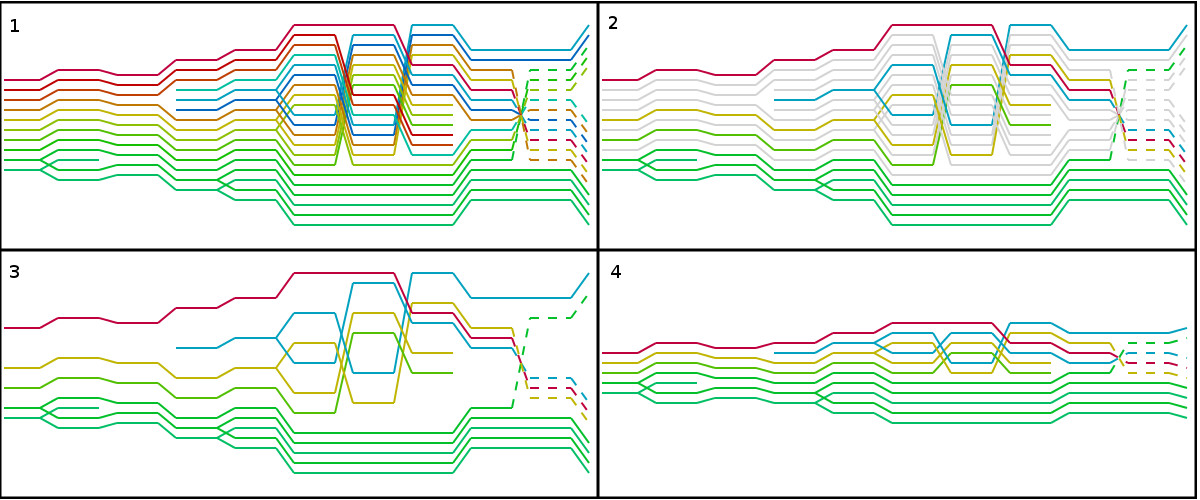
\includegraphics[width=1.1\textwidth]{images/optimalizacia}
\caption{Kroky optimalizácie}\label{obr:opt}
\end{figure}

